\documentclass[conference]{IEEEtran}

\usepackage{amsmath}
\usepackage{amssymb}
\usepackage{algorithm}
\usepackage{algorithmic}
\usepackage{booktabs}
\usepackage{graphicx}
\newcommand{\selected}[1]{\textbf{#1}}

\title{Appendix: Conservative Event-Level Timing Audit}
\author{}

\begin{document}
\maketitle

\appendices

\section{Conservative Event-Level Timing Audit}
\label{sec:appendix-alignment}

Each logged REFIT row provides a common timestamp but not the physical acquisition time of every individual meter reading.  Consequently, the recorded data cannot identify an exact, universal IAM-aggregate delay.  A single nearby aggregate step is also insufficient evidence for a shift, since an unmonitored load can produce that step.  We therefore describe the following procedure only as a conservative, diagnostic event-level audit; it is not part of the primary training or evaluation pipeline and does not claim physical synchronization.

Let $x_t$ and $P_{t,i}$ denote the recorded aggregate and appliance powers, respectively, and define $\Delta x_t=x_t-x_{t-1}$.  Consider a complete on period $[s,e)$ of appliance $i$, with a rising edge $a_i^{\uparrow}=P_{s,i}-P_{s-1,i}$ and a falling edge $a_i^{\downarrow}=P_{e-1,i}-P_{e,i}$.  Only events whose two appliance edges are at least $\max(40,0.3\tau_i)$~W are considered, where $\tau_i$ is the appliance on threshold.  We examine lags $\ell\in\{-2,-1,0,1,2\}$, corresponding to at most $\pm16$~s.  A lag is admissible only if both aggregate edges have the expected direction and sufficient magnitude:
\begin{equation}
\begin{aligned}
\Delta x_{s+\ell}&\geq\max(20,0.25a_i^{\uparrow}),\\
-\Delta x_{e+\ell}&\geq\max(20,0.25a_i^{\downarrow}).
\end{aligned}
\label{eq:alignment-gate}
\end{equation}
For every admissible lag, the two-edge discrepancy is
\begin{equation}
C_i(\ell)=\frac{1}{2}\left(
\frac{|\Delta x_{s+\ell}-a_i^{\uparrow}|}{\max(a_i^{\uparrow},40)}+
\frac{|{-\Delta x_{e+\ell}}-a_i^{\downarrow}|}{\max(a_i^{\downarrow},40)}
\right).
\label{eq:alignment-score}
\end{equation}
The selected lag is $\ell^*=\arg\min_{\ell}C_i(\ell)$, with zero lag preferred only when scores are tied.  We accept it only when $C_i(\ell^*)\leq0.75$, its margin over the next-best admissible lag is at least $0.20$, neither event boundary lies near a $\geq40$~W transition of another monitored target, and the shifted event would not overlap an existing on period.  Events failing any condition are left unchanged.

For an accepted non-zero lag, the aggregate is immutable.  Let $b_i$ be the median measured power in the nearby off samples and let $q_{t,i}=\max(P_{t,i}-b_i,0)$ within $[s,e)$.  The procedure moves the excess event profile as a whole:
\begin{equation}
\widetilde{P}_{t,i}=P_{t,i}-q_{t,i}\mathbf{1}_{[s,e)}(t)
+q_{t-\ell^*,i}\mathbf{1}_{[s+\ell^*,e+\ell^*)}(t),
\qquad \widetilde{x}_t=x_t.
\label{eq:event-shift}
\end{equation}
Thus $\sum_t\widetilde{P}_{t,i}=\sum_tP_{t,i}$ for every shifted event.  The associated binary on period is shifted by the same lag.  This preserves the recorded input and the appliance watt-sample energy; it does \emph{not} impose $x_t\geq\sum_iP_{t,i}$, because the measured target set is incomplete and the recorded aggregate must not be reconstructed using its labels.

The audit is a sensitivity analysis, not part of the retained training pipeline.  In our cross-house ablation it slightly changed local timing errors but did not consistently improve F1 or AP across the two held-out datasets.  The primary results therefore use the unshifted, mean-resampled recordings.  This distinction avoids treating a plausible timing hypothesis as ground truth.

\begin{algorithm}[!t]
\caption{Conservative two-edge event timing audit.}
\label{alg:alignment}
\begin{algorithmic}[1]
\REQUIRE 8-s aggregate $x_t$, appliance powers $P_{t,i}$, states $z_{t,i}$, thresholds $\tau_i$, and $L=2$ samples.
\ENSURE Audited appliance series $\widetilde{P}_{t,i}$ and states $\widetilde{z}_{t,i}$; aggregate $x_t$ is unchanged.
\STATE Set $\widetilde{P}_{t,i}\leftarrow P_{t,i}$ and $\widetilde{z}_{t,i}\leftarrow z_{t,i}$.
\FOR{each target appliance $i \in \{1,\ldots,M\}$}
    \FOR{each complete on period $[s,e)$ in $z_{t,i}$}
        \STATE Reject the event if an endpoint is unavailable, either appliance edge is below $\max(40,0.3\tau_i)$, or another monitored target has a transition of at least 40~W within $L$ samples of either boundary.
        \STATE Form the admissible lag set using \eqref{eq:alignment-gate}; discard candidates whose two relative edge errors exceed one.
        \IF{$C_i(\ell^*)\leq0.75$, the score margin is at least $0.20$, and the shifted interval does not overlap another ON interval}
            \STATE Move the excess profile and the complete state interval by $\ell^*$ using \eqref{eq:event-shift}.
        \ENDIF
    \ENDFOR
\ENDFOR
\STATE Verify $\sum_t\widetilde{P}_{t,i}=\sum_tP_{t,i}$ for every appliance and $x_t$ is bitwise unchanged.
\RETURN $x_t$, $\widetilde{P}_{t,i}$, and $\widetilde{z}_{t,i}$.
\end{algorithmic}
\end{algorithm}

\section{Loss-Function Ablation and Hyperparameter Robustness}
\label{sec:appendix-loss}

This appendix documents the loss-function study used to finalize MART-NILM. The retained objective removes relative energy loss (LRE), retaining on-state mean squared error (ON-MSE), off-state mean squared error (OFF-MSE), on-state masked temporal-difference mean squared error (Delta-MSE), a false-positive (FP) state penalty, and binary cross-entropy (BCE) state supervision. The selected coefficients are $w_{\mathrm{on}}=1.0$, $w_{\mathrm{off}}=0.5$, $w_{\Delta}=0.15$, $w_{\mathrm{FP}}=1.0$, and $\lambda_{\mathrm{state}}=0.8$; the BCE positive-weight cap is 12 and the task-balance clipping limit is 3.

\subsection{Objective Before and After LRE Removal}
\label{sec:appendix-loss-equations}

Let $Q_i$, $S_i$, and $r_i$ denote the base power loss, state loss, and detached appliance-wise balance ratio for appliance $i$, respectively.  With $\operatorname{sg}(\cdot)$ denoting stop-gradient, define
\begin{equation}
\begin{aligned}
Q_i &= \operatorname{MSE}_{i}+w_{\mathrm{on}}\operatorname{ON\text{-}MSE}_{i}
      +w_{\mathrm{off}}\operatorname{OFF\text{-}MSE}_{i}\\
&\quad +w_{\Delta}\operatorname{Delta\text{-}MSE}_{i},\\
S_i &= \operatorname{BCE}_{i}+w_{\mathrm{FP}}\operatorname{FP}_{i}.
\label{eq:appendix-power-state-components}
\end{aligned}
\end{equation}

The original objective used for the frozen Table~III reference was
\begin{equation}
\begin{aligned}
\mathcal{L}_{\mathrm{with\text{-}LRE}}
 &=\sum_{i=1}^{A}\left(Q_i+0.25\operatorname{LRE}_{i}\right)
 +0.8\sum_{i=1}^{A}S_i\operatorname{sg}\!\left(r_i^{\mathrm{old}}\right),\\
r_i^{\mathrm{old}}
 &=\operatorname{clip}\!\left(
 \frac{Q_i+0.25\operatorname{LRE}_{i}}{S_i},
 \frac{r^{\mathrm{old}}}{3},3r^{\mathrm{old}}\right),\\
r^{\mathrm{old}}
 &=\frac{\sum_i\left(Q_i+0.25\operatorname{LRE}_{i}\right)}{\sum_iS_i},\\
\operatorname{LRE}_{i}
 &=\frac{\sum_{t=1}^{T}|\widehat{P}_i(t)-P_i(t)|}
 {\sum_{t=1}^{T}P_i(t)+TP_0},\qquad P_0=10~\mathrm{W}.
\label{eq:appendix-objective-before}
\end{aligned}
\end{equation}
Here, $\operatorname{FP}_{i}$ is the mean squared state probability on true-OFF samples, and Delta-MSE is evaluated only on temporal pairs for which at least one sample is truly ON.  The terms MSE, ON-MSE, OFF-MSE, and Delta-MSE are evaluated in the standardized power space, whereas LRE is evaluated after conversion to watts.

The final retained objective is identical except that the relative-energy term is removed:
\begin{equation}
\begin{aligned}
\mathcal{L}_{\mathrm{final}}
 &=\sum_{i=1}^{A}Q_i+0.8\sum_{i=1}^{A}S_i\operatorname{sg}\!\left(r_i^{\mathrm{final}}\right),\\
r_i^{\mathrm{final}}
 &=\operatorname{clip}\!\left(\frac{Q_i}{S_i},\frac{r^{\mathrm{final}}}{3},3r^{\mathrm{final}}\right),\\
r^{\mathrm{final}}&=\frac{\sum_iQ_i}{\sum_iS_i},\\
Q_i &=\operatorname{MSE}_{i}+1.0\operatorname{ON\text{-}MSE}_{i}
 +0.5\operatorname{OFF\text{-}MSE}_{i}\\
&\quad +0.15\operatorname{Delta\text{-}MSE}_{i},\\
S_i &=\operatorname{BCE}_{i}+1.0\operatorname{FP}_{i}.
\label{eq:appendix-objective-after}
\end{aligned}
\end{equation}
Thus $w_E=0$ and neither LRE nor its denominator floor $P_0$ remains in the final model.  The ON-class BCE weight is still capped at 12, and $r_i$ retains the same clipping limit $c=3$.

All candidates retain the same data split, architecture, optimization schedule, post-processing, and evaluation pipeline. A term is removable or a replacement retainable only when it maintains or improves power-estimation and state-detection metrics in both test houses. Confirmed comparisons use three seeds (2026, 2027, and 2028); one-seed screens are used only to reject clearly weak neighbouring values.

\begin{table*}[!t]
\caption{Three-seed comparison before and after removal of LRE. Mean $\pm$ standard deviation. \selected{Selected} identifies the final objective. Removing LRE eliminates the denominator floor $P_0=10$~W while preserving performance.}
\label{tab:appendix-lre}
\centering\scriptsize
\begin{tabular}{llrrrrrl}
\toprule
Test house & Objective & MAE (W) & ON-MAE (W) & SAE (\%) & AP & F1 & Decision \\
\midrule
UK-DALE H2 & With LRE & $7.451\pm0.091$ & $176.669\pm7.675$ & $5.275\pm0.100$ & $0.926\pm0.008$ & $0.876\pm0.010$ & reject \\
UK-DALE H2 & \selected{Reference: no LRE} & $7.296\pm0.173$ & $175.296\pm6.924$ & $5.059\pm0.364$ & $0.926\pm0.010$ & $0.880\pm0.003$ & \selected{Selected} \\
REFIT H20 & With LRE & $10.798\pm0.355$ & $309.207\pm4.577$ & $5.893\pm0.390$ & $0.762\pm0.018$ & $0.716\pm0.016$ & reject \\
REFIT H20 & \selected{Reference: no LRE} & $10.931\pm0.174$ & $309.988\pm3.540$ & $5.959\pm0.233$ & $0.761\pm0.016$ & $0.717\pm0.003$ & \selected{Selected} \\
\bottomrule
\end{tabular}
\end{table*}

\begin{table*}[!t]
\caption{Loss-term removals relative to the no-LRE reference. Values are three-seed means unless marked \textit{screen} ($n=1$). The bold reference rows are retained; all removals are rejected under the cross-house decision rule. OFF-MAE audits background-power noise.}
\label{tab:appendix-terms}
\centering\scriptsize
\begin{tabular}{llrrrrrrl}
\toprule
Test house & Variant & $n$ & MAE (W) & ON-MAE (W) & OFF-MAE (W) & SAE (\%) & AP / F1 & Decision \\
\midrule
UK-DALE H2 & \selected{Reference} & 3 & 7.296 & 175.296 & 4.830 & 5.059 & .926 / .880 & \selected{Retain} \\
& No ON-MSE (\textit{screen}) & 1 & 8.217 & 310.657 & 4.115 & 6.136 & .920 / .874 & reject \\
& No OFF-MSE & 3 & 7.161 & 174.972 & 4.981 & 4.801 & .925 / .877 & reject \\
& No Delta-MSE & 3 & 7.472 & 202.025 & 4.796 & 5.251 & .924 / .865 & reject \\
& No FP penalty & 3 & 7.257 & 177.210 & 4.850 & 5.024 & .919 / .874 & reject \\
\midrule
REFIT H20 & \selected{Reference} & 3 & 10.931 & 309.988 & 7.550 & 5.959 & .761 / .717 & \selected{Retain} \\
& No ON-MSE (\textit{screen}) & 1 & 11.238 & 432.794 & 5.607 & 6.702 & .723 / .688 & reject \\
& No OFF-MSE & 3 & 11.184 & 307.688 & 8.212 & 6.200 & .755 / .715 & reject \\
& No Delta-MSE & 3 & 10.716 & 316.605 & 7.294 & 5.725 & .757 / .725 & reject \\
& No FP penalty & 3 & 10.858 & 304.509 & 7.572 & 5.944 & .760 / .716 & reject \\
\bottomrule
\end{tabular}
\end{table*}

\begin{figure*}[!t]
\centering
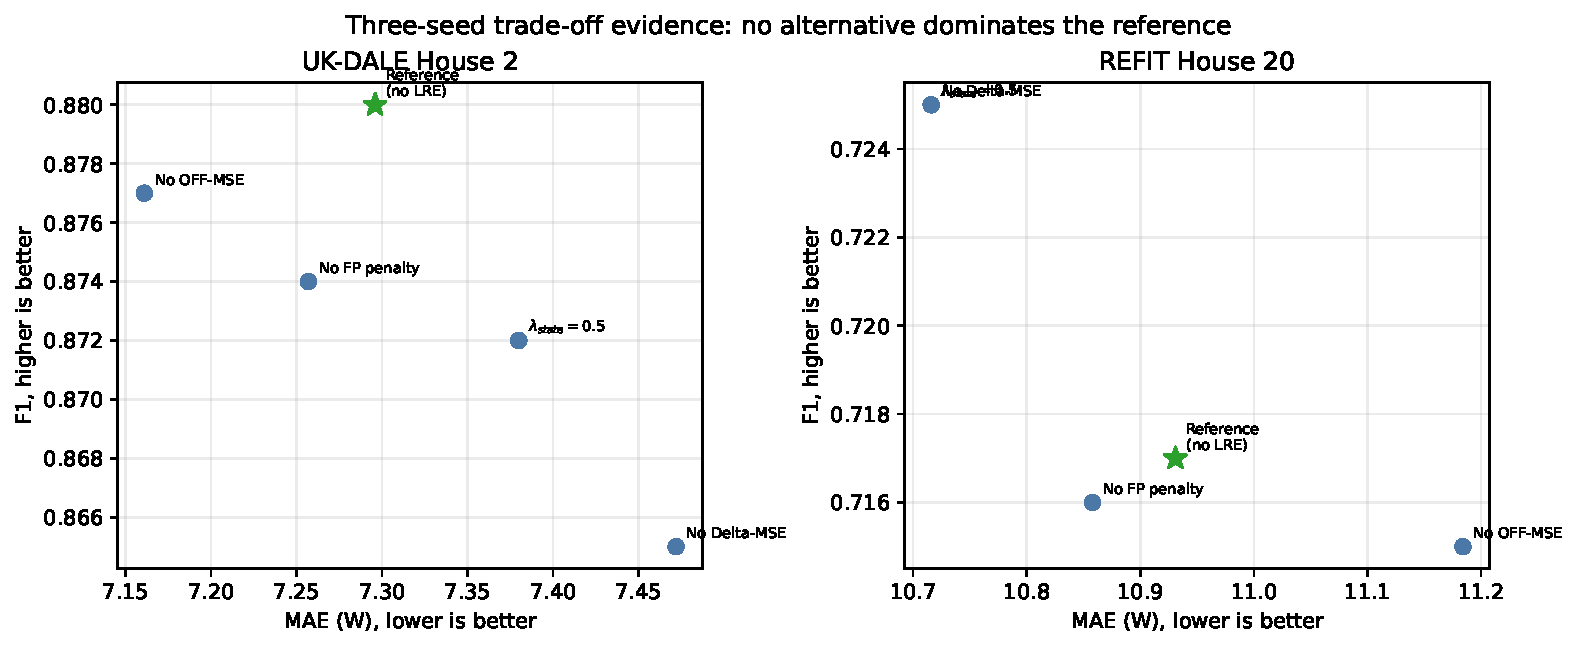
\includegraphics[width=0.92\textwidth]{appendix_figures/loss_pareto_confirmed.pdf}
\caption{Three-seed Pareto view of confirmed loss-term and weight alternatives. The no-LRE reference is retained because no alternative achieves lower MAE and higher F1 in both test houses.}
\label{fig:appendix-loss-pareto}
\end{figure*}

\begin{figure*}[!t]
\centering
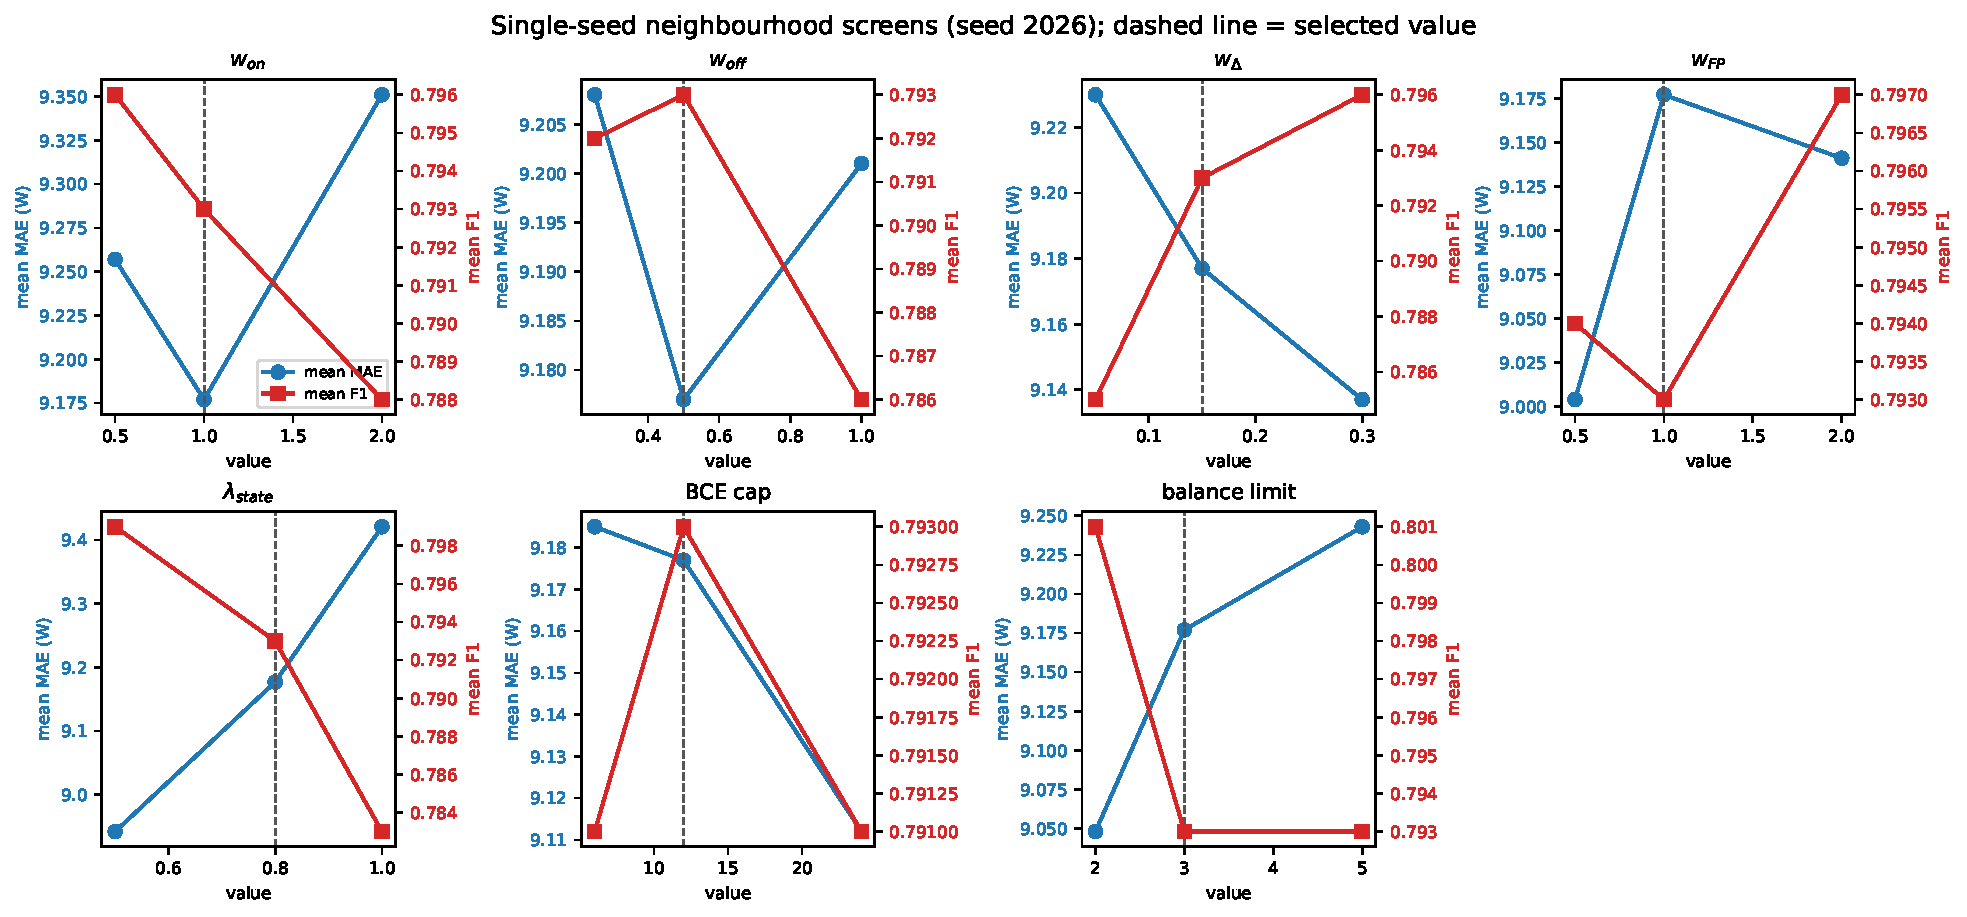
\includegraphics[width=\textwidth]{appendix_figures/loss_hyperparameter_screens.pdf}
\caption{Single-seed local hyperparameter screens. Blue: two-house mean MAE (lower is better). Red: two-house mean F1 (higher is better). Dashed lines mark the retained values.}
\label{fig:appendix-loss-screens}
\end{figure*}

\begin{table*}[!t]
\caption{Compact one-seed screen data. Each sequence follows increasing tested values and gives the arithmetic mean across UK-DALE H2 and REFIT H20. Bold identifies the retained setting, not the numerical minimum of an isolated metric; no candidate gives a strict joint power-state improvement.}
\label{tab:appendix-loss-screens}
\centering\scriptsize
\begin{tabular}{lclll}
\toprule
Parameter & Tested values & Two-house mean MAE (W) & Two-house mean F1 & Decision \\
\midrule
$w_{\mathrm{on}}$ & .5, \selected{1.0}, 2.0 & 9.257, 9.177, 9.351 & .796, .793, .788 & \selected{Retain 1.0} \\
$w_{\mathrm{off}}$ & .25, \selected{.5}, 1.0 & 9.208, 9.177, 9.201 & .792, .793, .786 & \selected{Retain .5} \\
$w_{\Delta}$ & .05, \selected{.15}, .30 & 9.230, 9.177, 9.137 & .785, .793, .796 & \selected{Retain .15} \\
$w_{\mathrm{FP}}$ & .5, \selected{1.0}, 2.0 & 9.004, 9.177, 9.141 & .794, .793, .797 & \selected{Retain 1.0} \\
$\lambda_{\mathrm{state}}$ & .5, \selected{.8}, 1.0 & 8.942, 9.177, 9.421 & .799, .793, .783 & \selected{Retain .8} \\
BCE cap & 6, \selected{12}, 24 & 9.185, 9.177, 9.112 & .791, .793, .791 & \selected{Retain 12} \\
Balance limit & 2, \selected{3}, 5 & 9.048, 9.177, 9.243 & .801, .793, .793 & \selected{Retain 3} \\
\bottomrule
\end{tabular}
\end{table*}

\subsection{OFF-MSE Waveform and Background-Noise Audit}
\label{sec:appendix-loss-waveforms}

Tables~\ref{tab:appendix-terms} and \ref{tab:appendix-term-seeds} quantify the OFF-MSE trade-off.  Figure~\ref{fig:appendix-loss-off-audit} provides a compact, matched-event audit: for each appliance, the reference and no-OFF-MSE predictions use the same saved REFIT H20 event and seed.  Blue is target power and dashed red is predicted power.  The complete background-range panels remain in the experiment archive; they are intentionally not reproduced here because the numerical OFF-MAE, AP, and F1 tables are the primary evidence.

\begin{figure*}[!t]
\centering
\begin{minipage}[t]{0.49\textwidth}
\centering
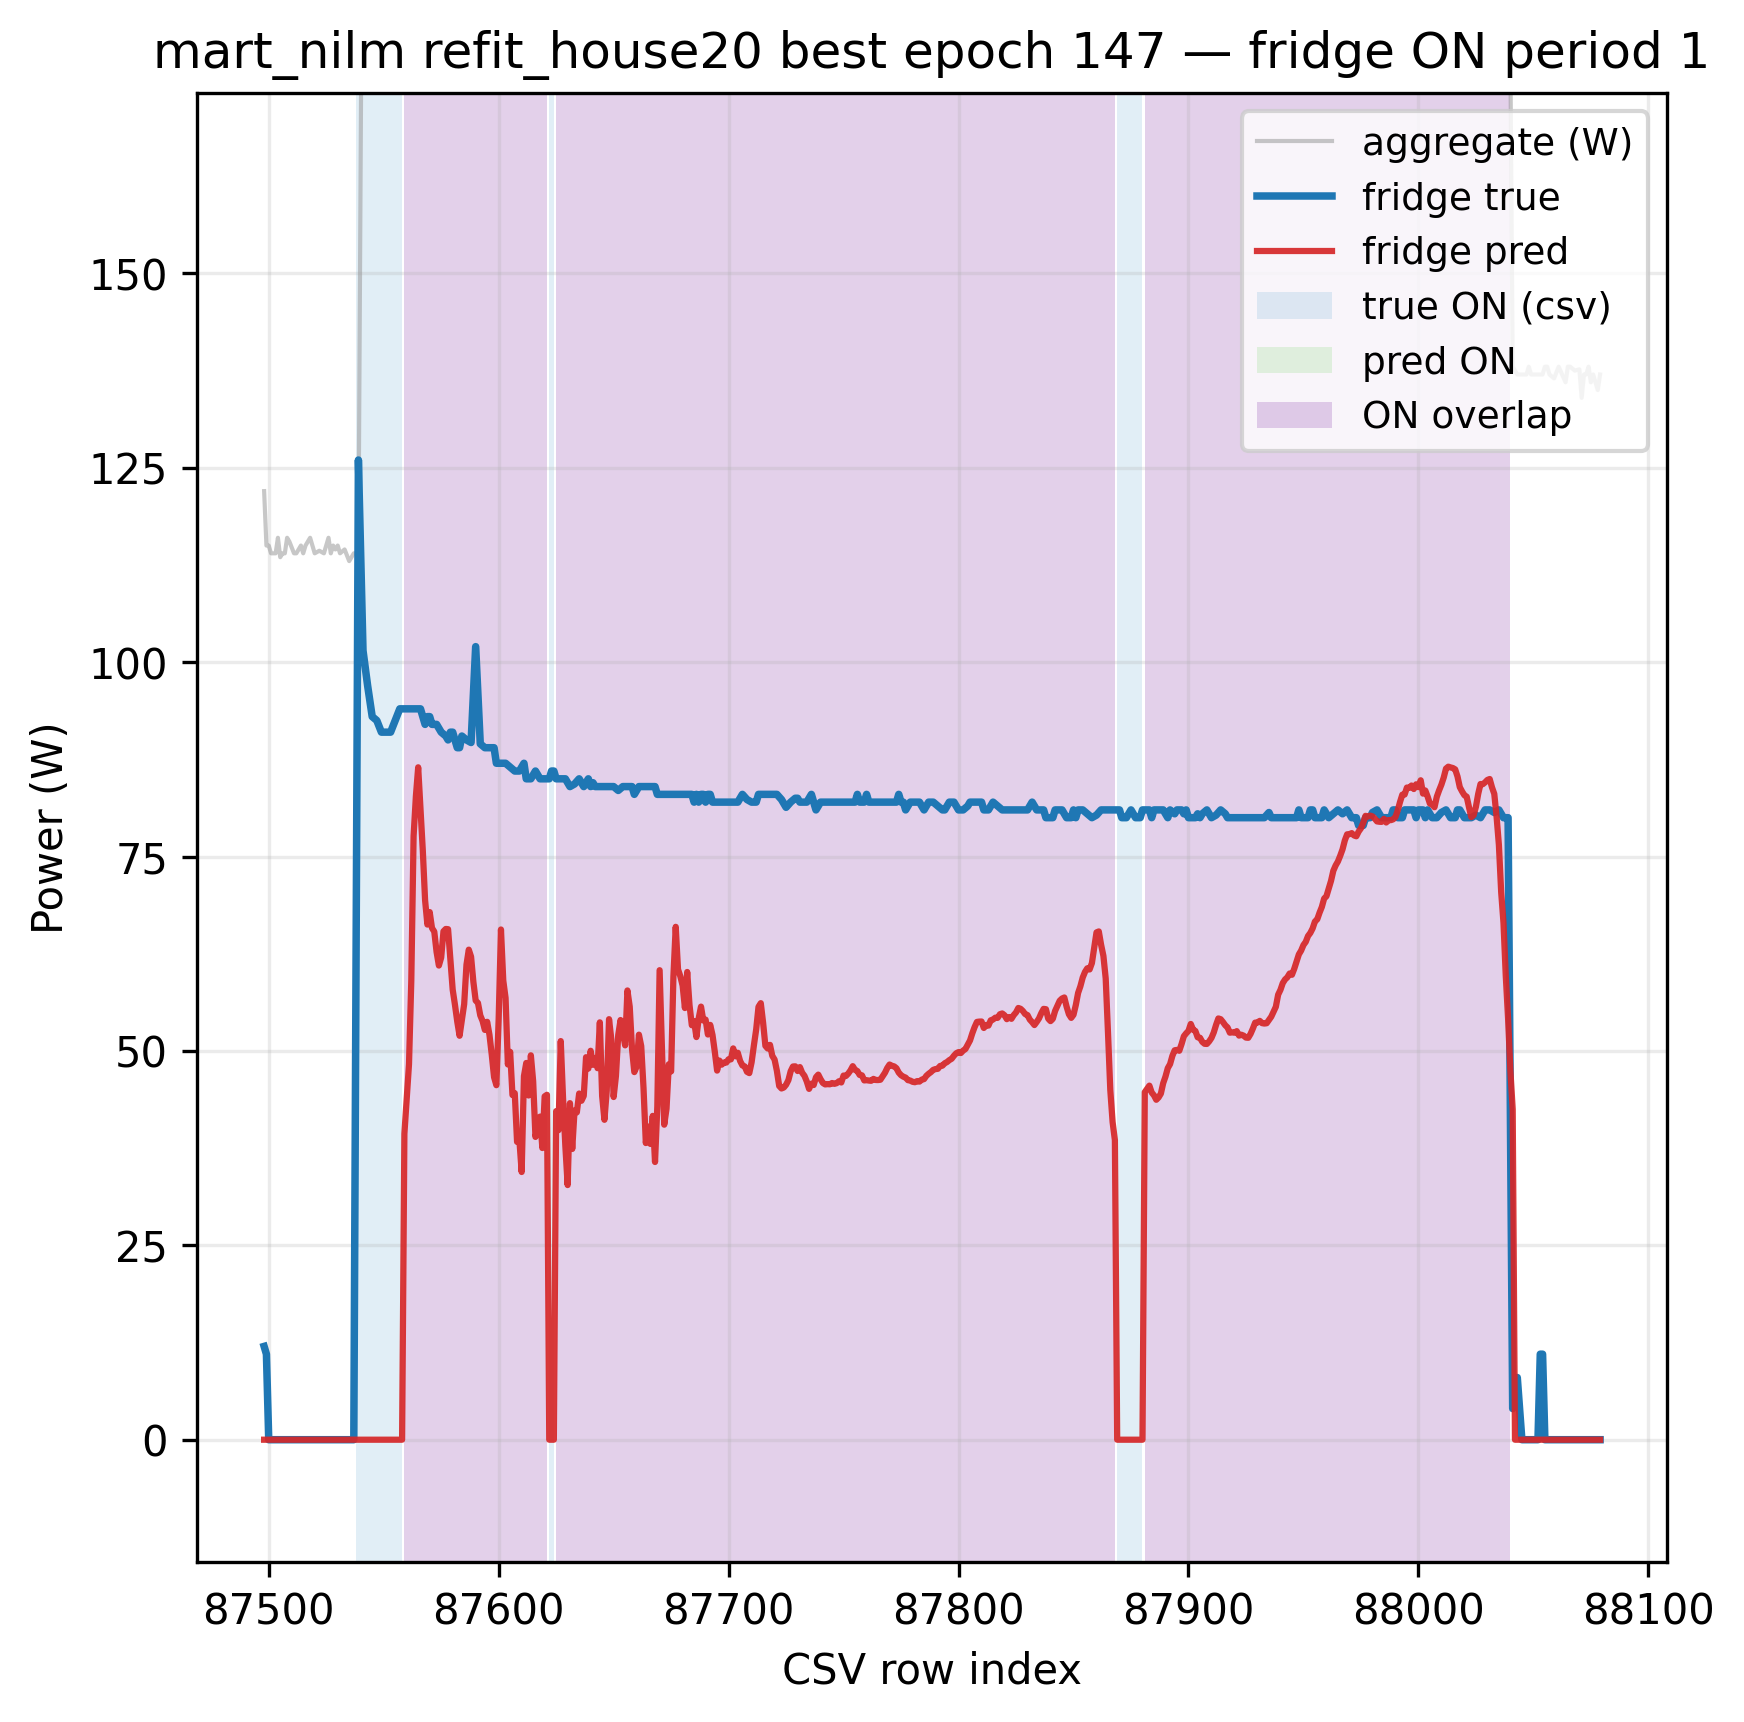
\includegraphics[width=\linewidth]{appendix_figures/loss_audit_reference_fridge.png}\\[-2pt]
\footnotesize (a) Fridge: retained reference
\end{minipage}\hfill
\begin{minipage}[t]{0.49\textwidth}
\centering
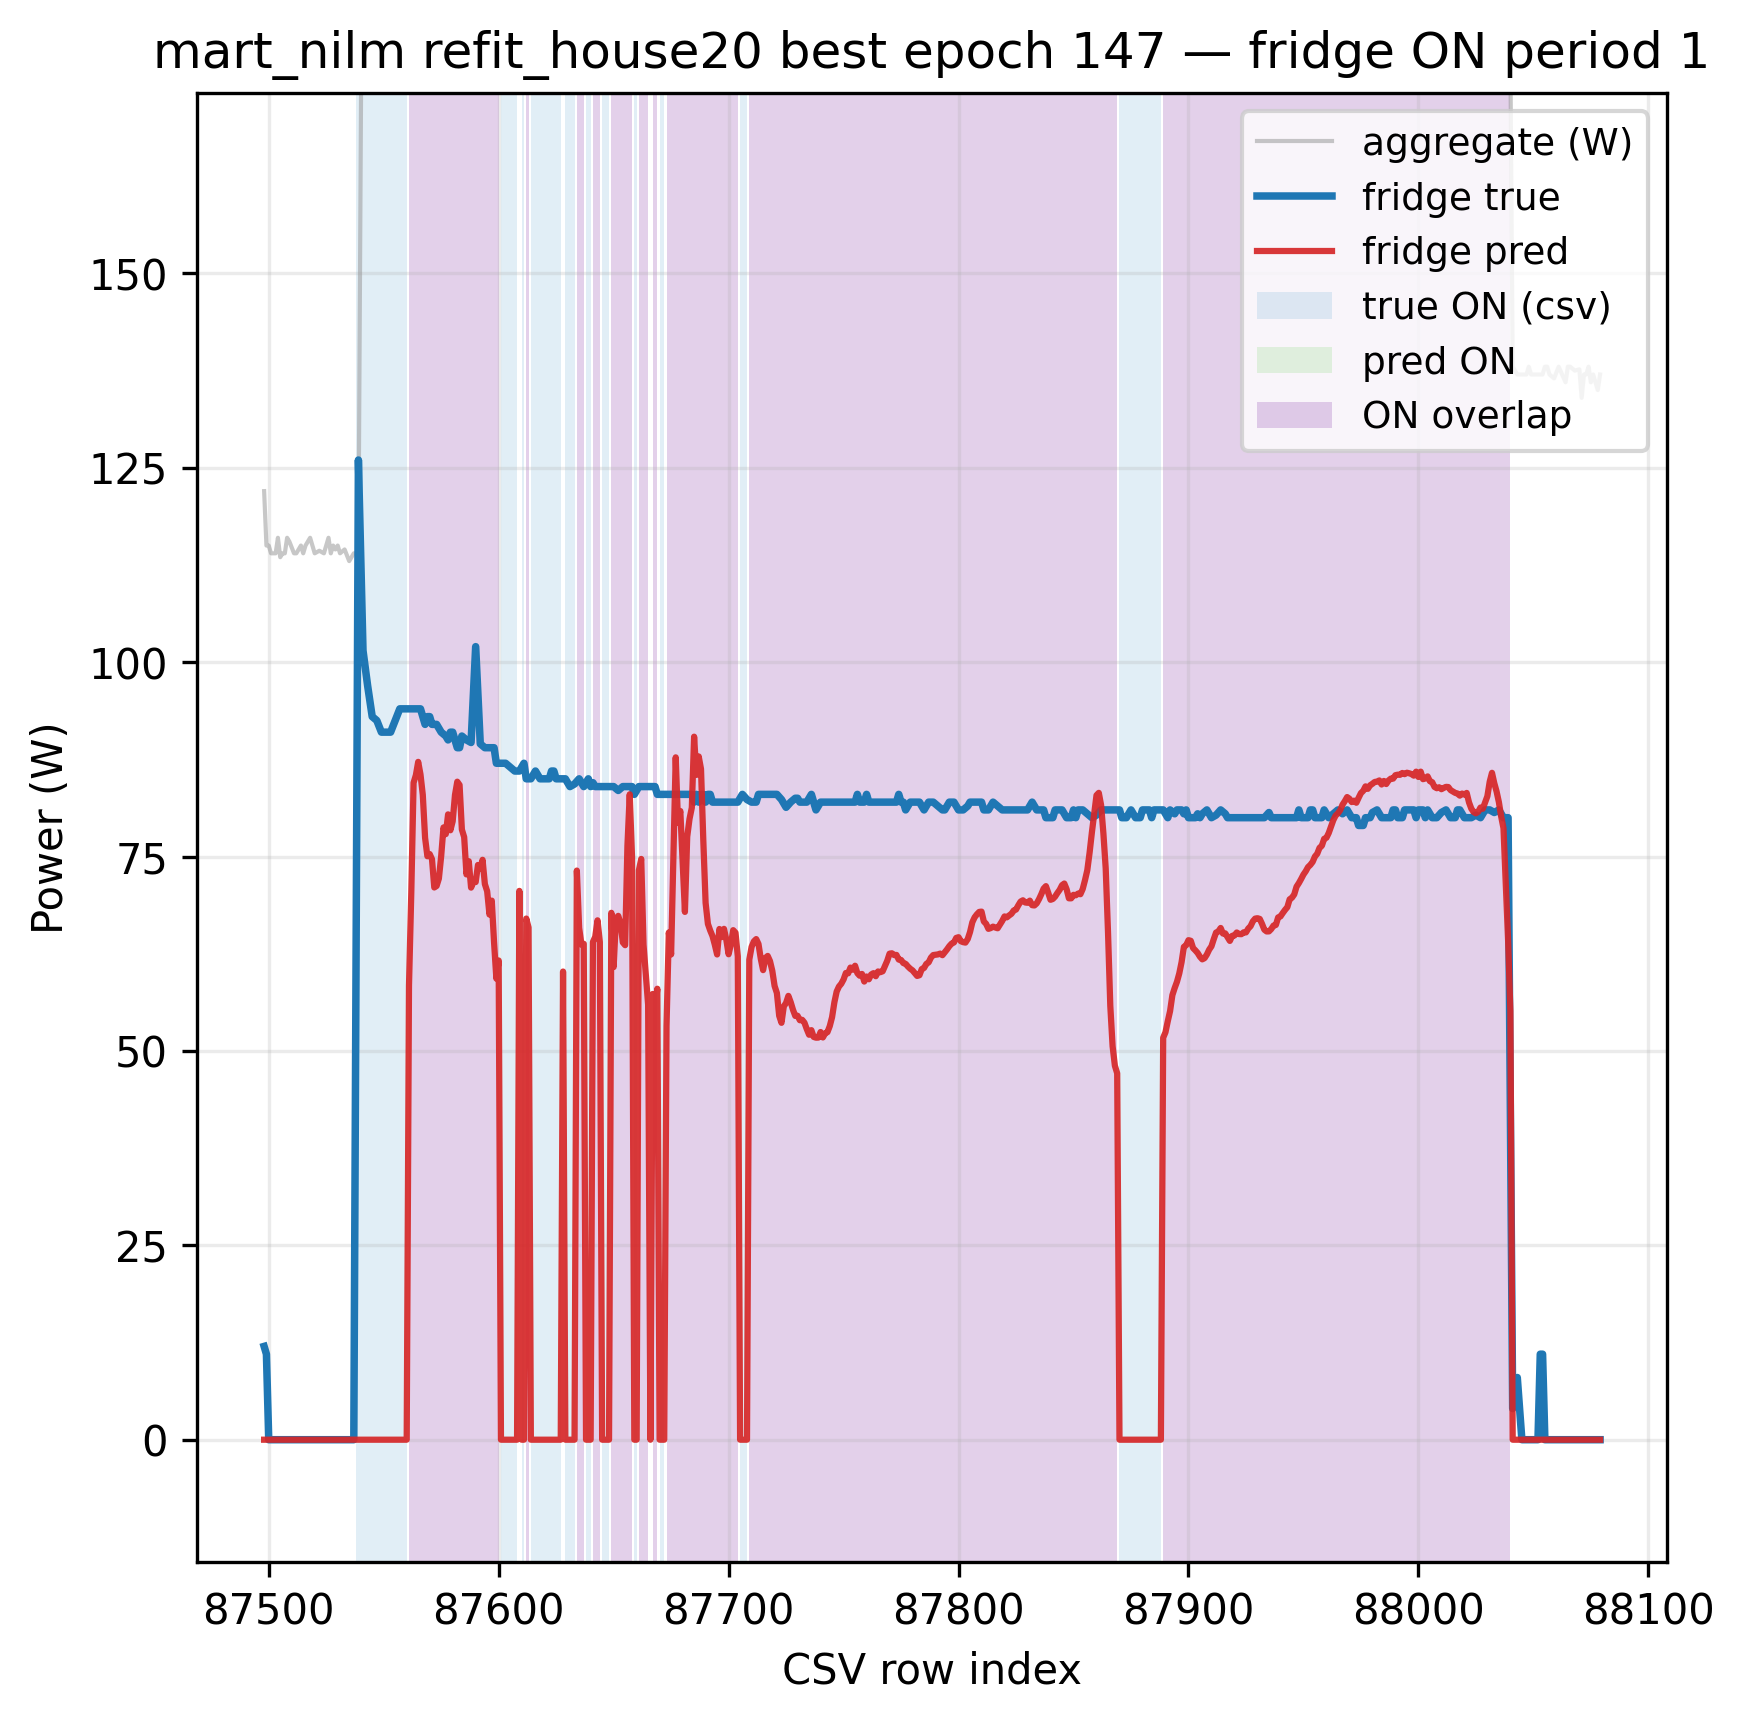
\includegraphics[width=\linewidth]{appendix_figures/loss_audit_no_off_fridge.png}\\[-2pt]
\footnotesize (b) Fridge: no OFF-MSE
\end{minipage}\par\smallskip
\begin{minipage}[t]{0.49\textwidth}
\centering
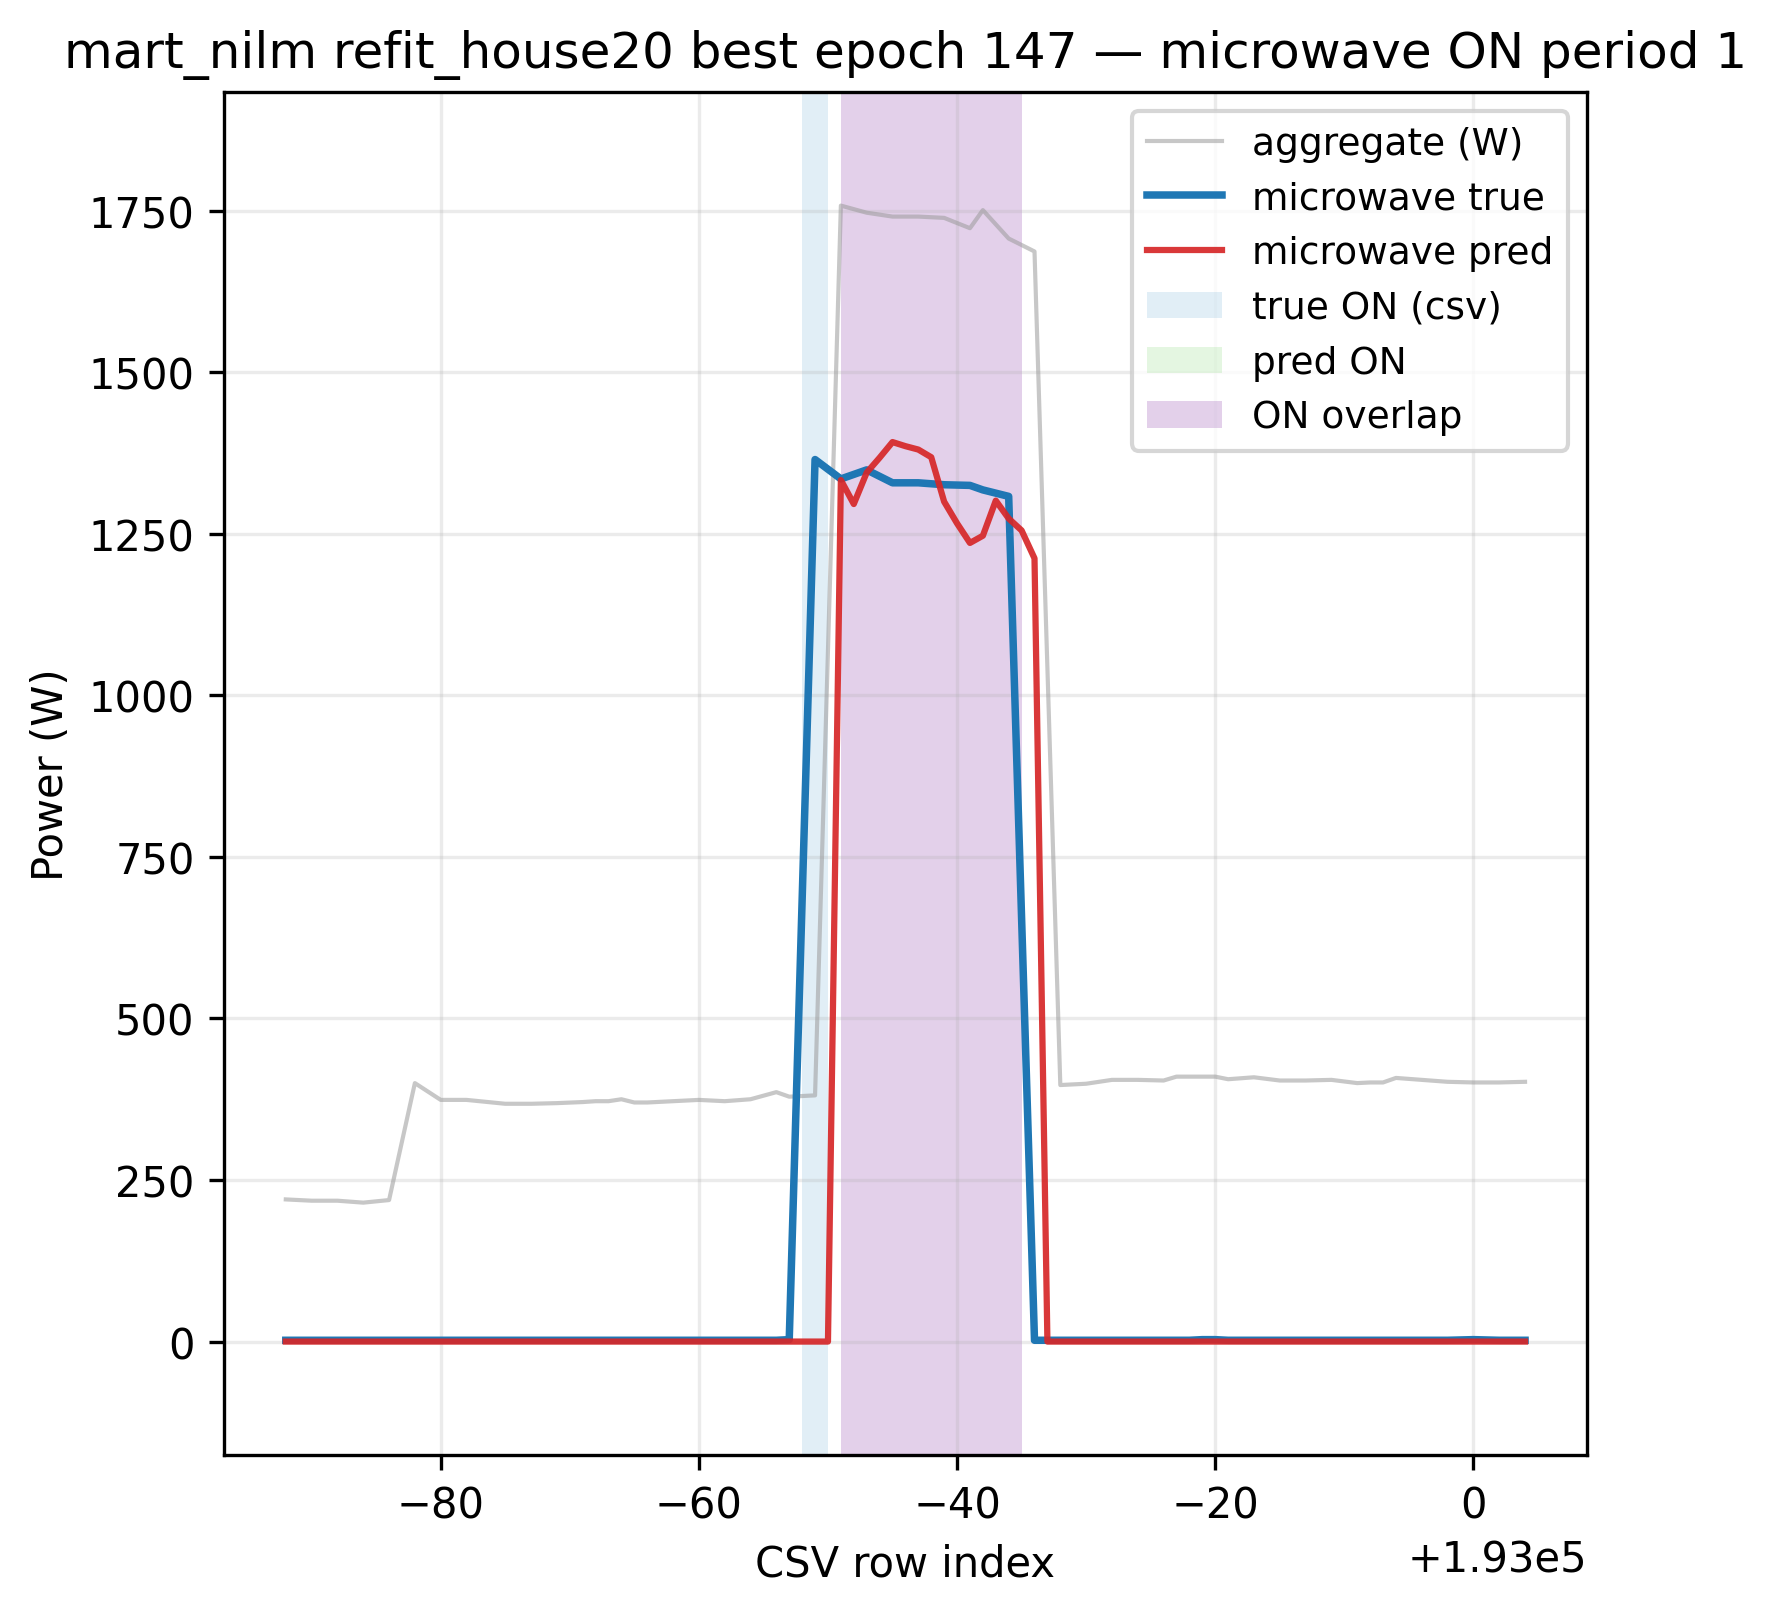
\includegraphics[width=\linewidth]{appendix_figures/loss_audit_reference_microwave.png}\\[-2pt]
\footnotesize (c) Microwave: retained reference
\end{minipage}\hfill
\begin{minipage}[t]{0.49\textwidth}
\centering
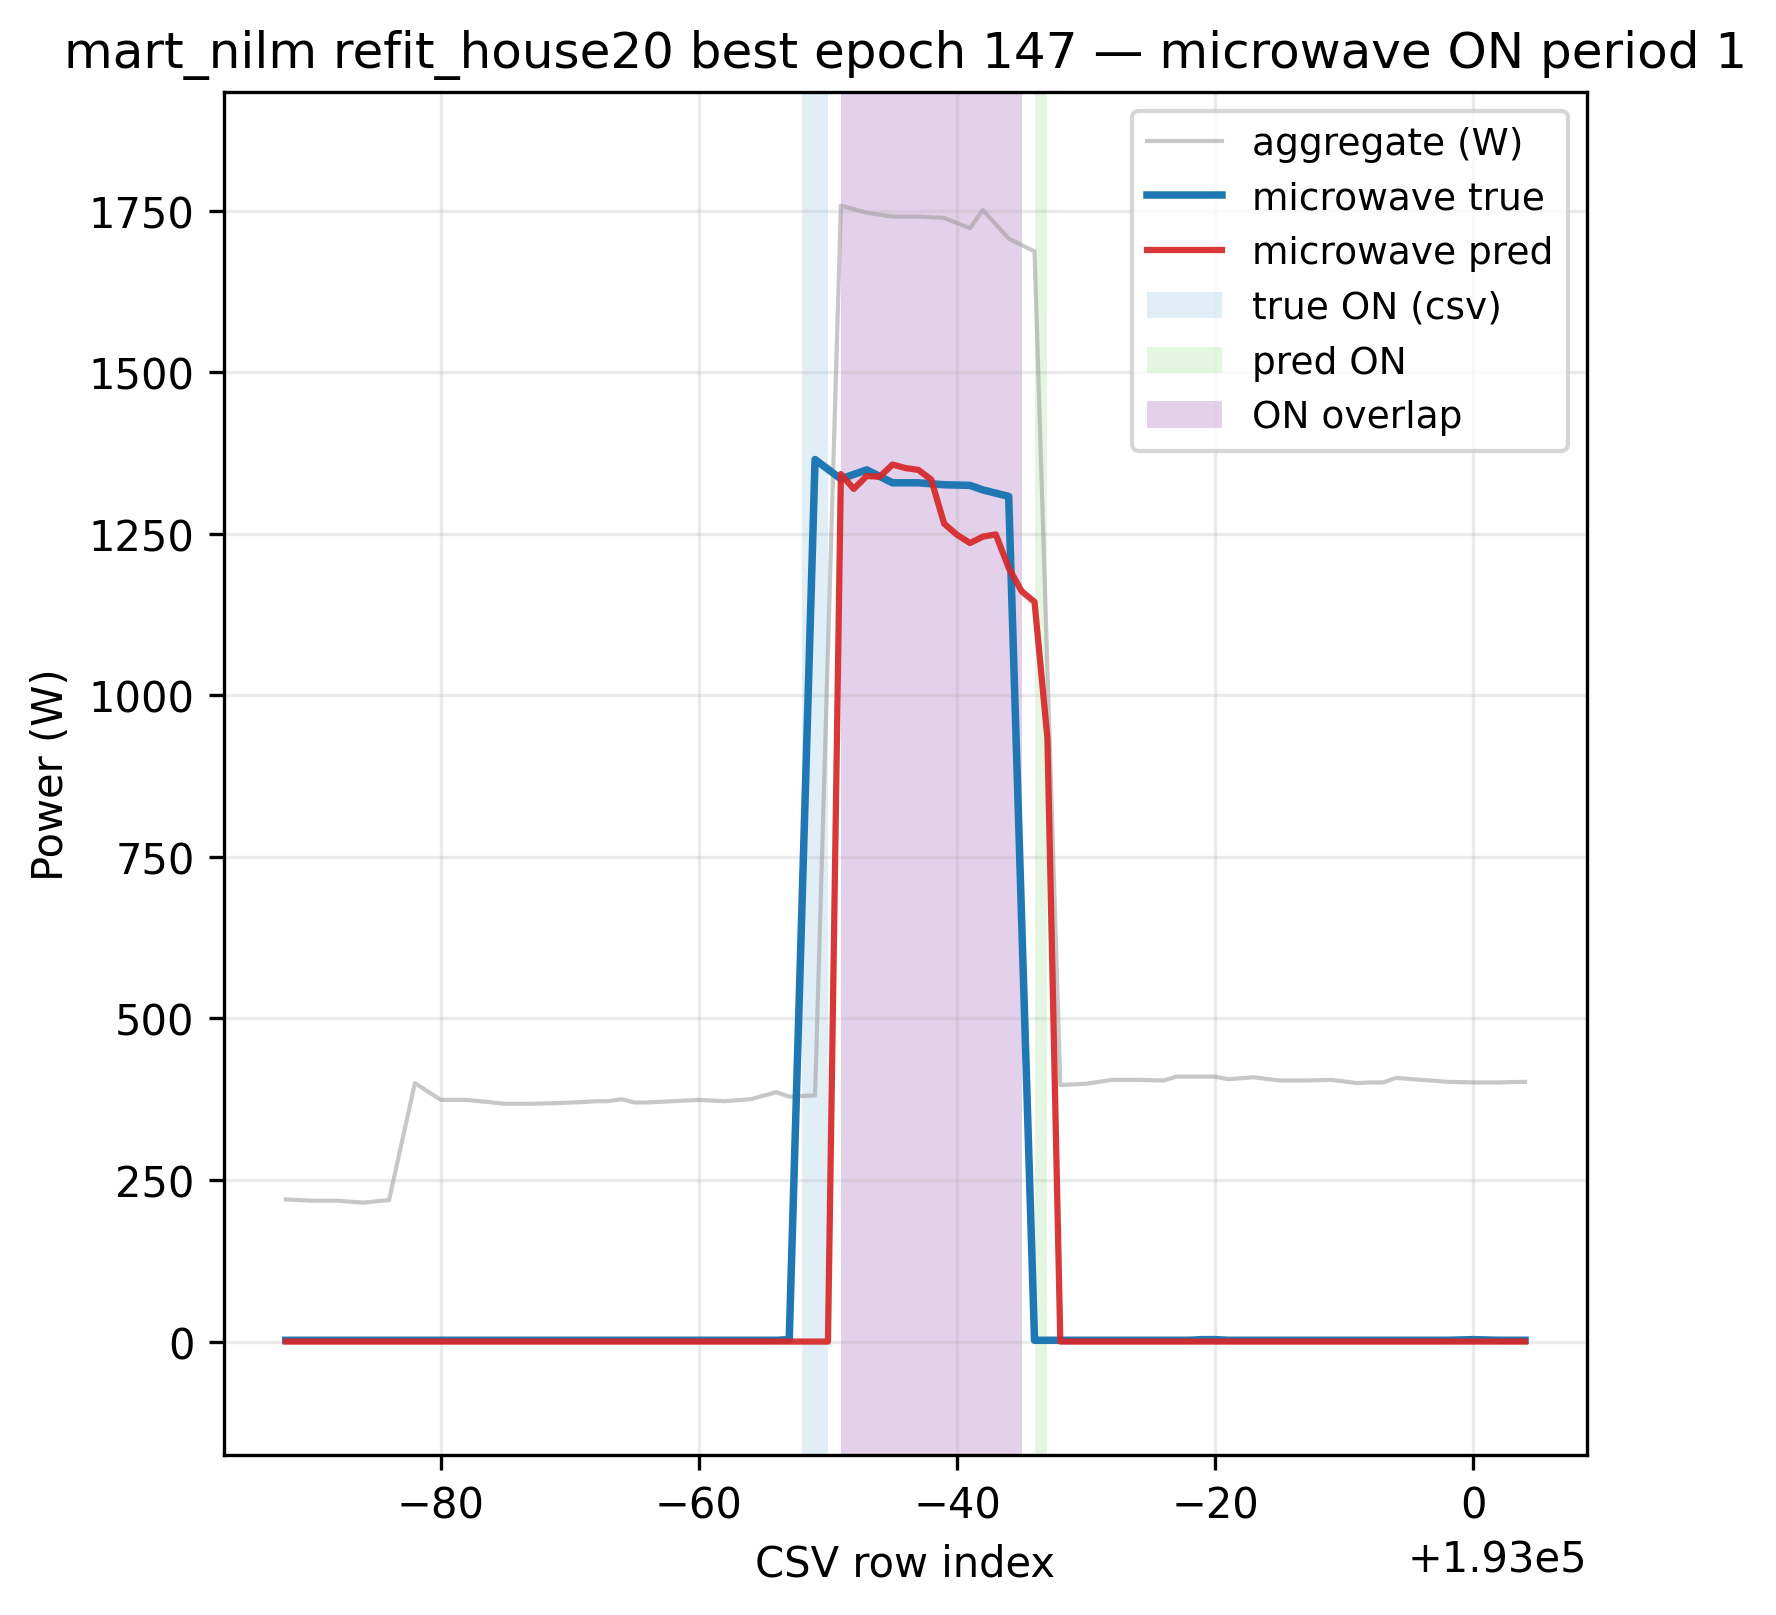
\includegraphics[width=\linewidth]{appendix_figures/loss_audit_no_off_microwave.png}\\[-2pt]
\footnotesize (d) Microwave: no OFF-MSE
\end{minipage}
\caption{Compact matched-event waveform audit for seed 2026 on REFIT H20.  Each column compares the same saved event under the retained no-LRE reference and no-OFF-MSE removal.}
\label{fig:appendix-loss-off-audit}
\end{figure*}

\subsection{Complete Seed-Level Test Results}
\label{sec:appendix-loss-complete-results}

For auditability, Tables~\ref{tab:appendix-lre-seeds}-\ref{tab:appendix-screen-refit} report every completed Table~III test result underlying the aggregate tables and response curves above.  Each row is the ``overall'' row in the saved metrics file; it is an appliance-averaged result, rather than a cherry-picked appliance result.  The retained no-LRE objective and the three confirmed term removals use seeds 2026, 2027, and 2028.  The remaining coefficient alternatives and the no-ON-MSE removal are one-seed exploratory screens (seed 2026), so they are reported as such and are not evidence of a statistically significant ranking.

\begin{table*}[!t]
\caption{Complete three-seed Table~III results for the relative-energy-loss (LRE) comparison.  Each seed was evaluated at the validation-selected checkpoint.  MAE, ON-MAE, and OFF-MAE are in W; SAE is in \%.}
\label{tab:appendix-lre-seeds}
\centering\scriptsize
\begin{tabular}{llrrrrrr}
\toprule
Test house & Objective / seed & MAE & ON-MAE & OFF-MAE & SAE & AP & F1 \\
\midrule
UK-DALE H2 & With LRE / 2026 & 7.407 & 170.046 & 4.622 & 5.287 & .935 & .879 \\
& With LRE / 2027 & 7.390 & 185.080 & 4.725 & 5.169 & .920 & .884 \\
& With LRE / 2028 & 7.555 & 174.880 & 4.831 & 5.368 & .924 & .865 \\
& \selected{No LRE / 2026} & \selected{7.338} & \selected{167.554} & 4.772 & 5.224 & \selected{.938} & .877 \\
& \selected{No LRE / 2027} & \selected{7.106} & \selected{177.439} & 4.851 & \selected{4.641} & .921 & \selected{.883} \\
& \selected{No LRE / 2028} & \selected{7.445} & 180.896 & \selected{4.724} & \selected{5.311} & .920 & \selected{.880} \\
\midrule
REFIT H20 & With LRE / 2026 & 11.133 & 310.321 & 7.513 & 6.246 & .742 & .697 \\
& With LRE / 2027 & 10.836 & 313.124 & 7.412 & 5.960 & .777 & .722 \\
& With LRE / 2028 & \selected{10.426} & 304.176 & 6.723 & \selected{5.474} & .768 & .728 \\
& \selected{No LRE / 2026} & 11.002 & 309.573 & 7.745 & 6.064 & .746 & .716 \\
& \selected{No LRE / 2027} & 11.058 & \selected{306.674} & 7.965 & 6.120 & \selected{.777} & .720 \\
& \selected{No LRE / 2028} & 10.732 & 313.718 & 6.985 & 5.692 & .760 & .714 \\
\bottomrule
\end{tabular}
\end{table*}

\begin{table*}[!t]
\caption{Complete seed-level test outcomes for loss-term removals.  All rows use no LRE.  No ON-MSE is a one-seed rejection screen; the other removals are three-seed comparisons.}
\label{tab:appendix-term-seeds}
\centering\scriptsize
\begin{tabular}{llrrrrrr}
\toprule
Test house & Variant / seed & MAE & ON-MAE & OFF-MAE & SAE & AP & F1 \\
\midrule
UK-DALE H2 & No ON-MSE / 2026 & 8.217 & 310.657 & 4.115 & 6.136 & .920 & .874 \\
& No OFF-MSE / 2026 & 7.188 & 165.192 & 4.901 & 5.080 & .940 & .877 \\
& No OFF-MSE / 2027 & 7.108 & 184.424 & 5.036 & 4.519 & .918 & .872 \\
& No OFF-MSE / 2028 & 7.187 & 175.301 & 5.005 & 4.803 & .918 & .882 \\
& No Delta-MSE / 2026 & 7.448 & 169.168 & 4.772 & 5.326 & .936 & .875 \\
& No Delta-MSE / 2027 & 7.480 & 224.361 & 4.813 & 5.211 & .916 & .858 \\
& No Delta-MSE / 2028 & 7.487 & 212.547 & 4.803 & 5.217 & .919 & .862 \\
& No FP penalty / 2026 & 7.126 & 165.983 & 4.760 & 4.954 & .932 & .879 \\
& No FP penalty / 2027 & 7.333 & 200.302 & 4.853 & 5.046 & .909 & .873 \\
& No FP penalty / 2028 & 7.313 & 165.344 & 4.938 & 5.073 & .916 & .869 \\
\midrule
REFIT H20 & No ON-MSE / 2026 & 11.238 & 432.794 & 5.607 & 6.702 & .723 & .688 \\
& No OFF-MSE / 2026 & 11.146 & 303.052 & 7.904 & 6.178 & .756 & .713 \\
& No OFF-MSE / 2027 & 11.242 & 313.026 & 8.641 & 6.274 & .760 & .724 \\
& No OFF-MSE / 2028 & 11.163 & 306.986 & 8.091 & 6.148 & .749 & .709 \\
& No Delta-MSE / 2026 & 10.724 & 301.089 & 7.419 & 5.751 & .758 & .721 \\
& No Delta-MSE / 2027 & 10.635 & 328.301 & 7.072 & 5.645 & .775 & .740 \\
& No Delta-MSE / 2028 & 10.790 & 320.424 & 7.391 & 5.780 & .739 & .715 \\
& No FP penalty / 2026 & 10.965 & 308.647 & 7.770 & 6.196 & .748 & .696 \\
& No FP penalty / 2027 & 10.938 & 303.071 & 7.571 & 5.881 & .769 & .730 \\
& No FP penalty / 2028 & 10.670 & 301.809 & 7.374 & 5.756 & .762 & .722 \\
\bottomrule
\end{tabular}
\end{table*}

\begin{table*}[!t]
\caption{Complete seed-2026 Table~III screen results for UK-DALE H2.  ``Setting'' gives the tested value; the reference is the no-LRE objective.  All non-reference rows are exploratory one-seed screens and were rejected.}
\label{tab:appendix-screen-ukdale}
\centering\scriptsize
\begin{tabular}{llrrrrrr}
\toprule
Screen & Setting & MAE & ON-MAE & OFF-MAE & SAE & AP & F1 \\
\midrule
\selected{Reference} & \selected{retained} & \selected{7.338} & \selected{167.554} & 4.772 & 5.224 & .938 & .877 \\
$w_{\mathrm{on}}$ & .5 & 7.480 & 180.087 & 4.611 & 5.406 & .940 & .881 \\
$w_{\mathrm{on}}$ & 2.0 & 7.256 & 163.440 & 5.009 & 5.029 & .938 & .874 \\
$w_{\mathrm{off}}$ & .25 & 7.221 & 165.462 & 4.881 & 5.086 & .933 & .872 \\
$w_{\mathrm{off}}$ & 1.0 & 7.555 & 184.348 & 4.590 & 5.621 & .937 & .879 \\
$w_{\Delta}$ & .05 & 7.273 & 171.901 & 4.821 & 5.078 & .925 & .870 \\
$w_{\Delta}$ & .30 & 7.332 & 172.906 & 4.778 & 5.214 & .940 & .874 \\
$w_{\mathrm{FP}}$ & .5 & 7.365 & 173.195 & 4.763 & 5.298 & .937 & .870 \\
$w_{\mathrm{FP}}$ & 2.0 & 7.262 & 191.412 & 4.806 & 5.079 & .938 & .879 \\
$\lambda_{\mathrm{state}}$ & .5 & 7.159 & 177.347 & 4.896 & 4.941 & .936 & .877 \\
$\lambda_{\mathrm{state}}$ & 1.0 & 7.124 & 196.239 & 4.757 & 4.880 & .943 & .890 \\
BCE cap & 6 & 7.240 & 172.077 & 4.669 & 5.189 & .934 & .883 \\
BCE cap & 24 & 7.264 & 162.198 & 4.821 & 5.088 & .933 & .870 \\
Balance limit & 2 & 7.269 & 168.540 & 4.772 & 5.153 & .938 & .883 \\
Balance limit & 5 & 7.391 & 169.294 & 4.821 & 5.237 & .935 & .873 \\
\bottomrule
\end{tabular}
\end{table*}

\begin{table*}[!t]
\caption{Complete seed-2026 Table~III screen results for REFIT H20.  The rows correspond exactly to Table~\ref{tab:appendix-screen-ukdale}; all non-reference rows are exploratory one-seed screens and were rejected.}
\label{tab:appendix-screen-refit}
\centering\scriptsize
\begin{tabular}{llrrrrrr}
\toprule
Screen & Setting & MAE & ON-MAE & OFF-MAE & SAE & AP & F1 \\
\midrule
\selected{Reference} & \selected{retained} & \selected{11.002} & \selected{309.573} & 7.745 & 6.064 & .746 & .716 \\
$w_{\mathrm{on}}$ & .5 & 11.034 & 307.730 & 7.348 & 6.264 & .747 & .711 \\
$w_{\mathrm{on}}$ & 2.0 & 11.445 & 299.844 & 8.551 & 6.515 & .745 & .702 \\
$w_{\mathrm{off}}$ & .25 & 11.195 & 299.545 & 8.082 & 6.160 & .754 & .711 \\
$w_{\mathrm{off}}$ & 1.0 & 10.846 & 308.349 & 7.047 & 6.063 & .740 & .693 \\
$w_{\Delta}$ & .05 & 11.186 & 313.238 & 7.829 & 6.377 & .747 & .699 \\
$w_{\Delta}$ & .30 & 10.942 & 317.410 & 7.727 & 5.911 & .744 & .717 \\
$w_{\mathrm{FP}}$ & .5 & 10.643 & 320.823 & 7.335 & 5.680 & .748 & .717 \\
$w_{\mathrm{FP}}$ & 2.0 & 11.019 & 318.870 & 7.756 & 6.123 & .750 & .715 \\
$\lambda_{\mathrm{state}}$ & .5 & 10.724 & 311.233 & 7.464 & 5.786 & .766 & .720 \\
$\lambda_{\mathrm{state}}$ & 1.0 & 11.717 & 319.303 & 8.066 & 6.631 & .731 & .675 \\
BCE cap & 6 & 11.130 & 314.440 & 7.449 & 6.195 & .734 & .698 \\
BCE cap & 24 & 10.959 & 307.008 & 7.585 & 5.907 & .751 & .711 \\
Balance limit & 2 & 10.826 & 304.409 & 7.623 & 5.952 & .751 & .718 \\
Balance limit & 5 & 11.094 & 301.253 & 7.715 & 6.036 & .743 & .712 \\
\bottomrule
\end{tabular}
\end{table*}

State metrics alone are insufficient: removing OFF-MSE raises REFIT OFF-MAE from 7.55 to 8.21~W despite similar F1 (0.717 to 0.715), and removing Delta-MSE raises UK-DALE ON-MAE from 175.30 to 202.03~W despite AP changing only from 0.926 to 0.924. The evidence therefore supports the compact retained objective within the tested ranges, not a claim of formal global hyperparameter optimality.

\end{document}
